\documentclass[a4paper, 12pt,oneside]{article} 
%\documentclass[a4paper, 12pt,oneside,draft]{article} 
%\usepackage{preamble}
\usepackage{preamble_bis}
%--------------------- ACTUAL FILE ---------------------- %
\begin{document} 
%%%
	\begin{titlepage}
    \newcommand{\HRule}{\rule{\linewidth}{0.5mm}} % Defines a new command for the horizontal lines, change thickness here
    
    \center  % Center everything on the page
     
    %----------------------------------------------------------------------------------------
    %   HEADING SECTIONS
    %----------------------------------------------------------------------------------------
    
    \vspace{3cm}
    \textsc{\LARGE École polytechnique fédérale de Lausanne}\\[1.5cm] % Name of your university/college
    
    \textsc{\Large Project N$^\circ$2 Report}\\[0.5cm] % Major heading such as course name
    \textsc{\large Randomized Nystr\"om
    }\\[0.5cm] % Minor heading such as course title
    
    %----------------------------------------------------------------------------------------
    %   TITLE SECTION
    %----------------------------------------------------------------------------------------
    
    \HRule \\[0.4cm] % line above and under the title
    
    
    % Title of your document
    
    \HRule \\[1.5cm]
     
    %----------------------------------------------------------------------------------------
    %   AUTHOR SECTION
    %----------------------------------------------------------------------------------------
    
    \begin{minipage}{0.4\textwidth}
    \begin{flushleft} \large
    
    \emph{Authors:}\\
    Tara \textsc{Fjellman}\\
    Amal \textsc{Seddas}\\
    
    
    
    
    \end{flushleft}
    \end{minipage}
    ~
    \begin{minipage}{0.4\textwidth}
    \begin{flushright} \large
    
    \emph{Professor:} \\
    Laura \textsc{Grigori
     }\\
    \end{flushright}
    \end{minipage}\\[10cm]
    %
    
    
    %----------------------------------------------------------------------------------------
    %   LOGO SECTION
    %----------------------------------------------------------------------------------------
    
    
\includegraphics[width=0.4\linewidth]{Logo-1 .pdf}\\[1cm] 
    % Include a department/university logo - this will require the graphicx package
     
    %----------------------------------------------------------------------------------------
    
    \vfill % Fill the rest of the page with whitespace
    
    \end{titlepage} 
	% Add titlepage
	\clearpage
	\tableofcontents
	\thispagestyle{empty}
	% Add table of contents
	\clearpage
	\pagenumbering{arabic}
	\setcounter{page}{1}

	\section{Introduction}
		\lipsum[1]
	\section{Algorithms}
        \subsection{Sketching Matrices}
        \subsection{Randomized Nyström low rank approximation}
	\section{Stability analysis}
		- bullet points about comments to include 
	\section{Parallelisation}
	\section{Experimental procedure}
		- averaging to increase precision of results
		- when running in parallel, was simited by number of cores $p=2^{2s}$ with $s\in\mathbb{N}$ (due to perfect square constraint of the paralelised matrix multiplication and the SHRT algorithm using the Hadamard transform), so we ran results for 1,4,16,64
		- ran results on the Helvetios cluster 
		- $k$ was taken often around $n/20$ as we deemed this value relevant for real applications
		- n was made vary as powers of $2$ due to the Hadamard transformation while $l$ was taken logaritmically spaced just to make the visuals more easy to interpret  
	\section{Algorithm Performance}
        \subsection{Sequential Performance}
		- in general (both plots) observe that k rank approximation represents minority of runtime (as expected as of order $k^3 +nk^2$). Indeed for shown examples represents at most 10\%. This would be different if one were to take big values of $k$. Also does not really seem to depend on sketching method which makes sense given the computations are the same regardless of which sketching method was used to obtain the B and C matrices
		\begin{figure}[htb]       
			\centering             
				\vspace{0em}
				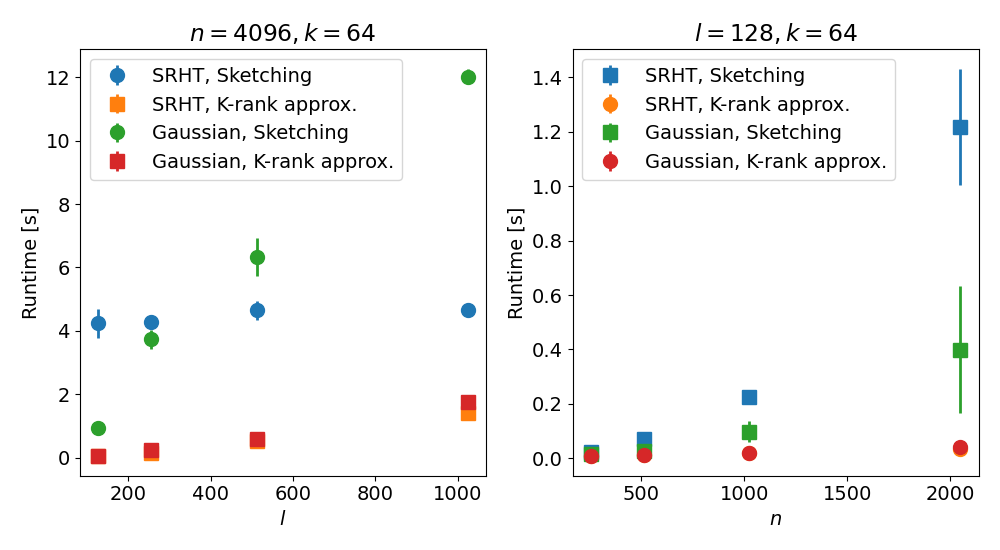
\includegraphics[width=.975\textwidth]{runtimes_l_n_variation}
				\caption{Runtimes associated to the tested sketching methods : as a function of $l$ (left) and as a function of $n$ (right). Runtimes are broken down in that associated to the computation of $A\Omega,\Omega^T A\Omega$ and that associated to the computation of the $k$ rank approximation.}
				\label{fig:runtimes-l-n-variation}
		\end{figure}

		- different behaviours as a function of l and n : as a function of l SRHT looks almost flat, having really slow increase, while gaussian increases steadily given its complexity is or order $nl^2 + ln^2$. This gives advantage for SRHT if we are embedding "dense spaces" as it scales much better than gaussian as function of l. For n : both algos show significant increase, but SRHT shows faster runtime growth. This makes sense due to extra $\log_2(n)$ term in its complexity. This would give advantage to gaussian sketching if we are dealing with sparse information within really high dimensional spaces.
		- 
        \subsection{Parallel Performance}
		- selected $l=n/64$ given we are using TSQR for the QR factorisation and we need the matrix to be tall-skinny to actually observe a speed-up. To have a good speed-up for a bigger $l$, while keeping numerical stability for ill-conditionned matrices another algo should be used.

		- for small example : some speed-up is observed as a function of number of cores but communication costs are non neglectable and even dominate the total runtime for p=64. This is expected as the computation is rather small to be run in parallel. The runtimes for the k-rank are the most affected as these represented the smallest part of the computation to start with. for the specific values selected the gaussian sketching is faster (indeed $l$ is taken only as a small fraction of $n$).

		\begin{figure}[htb]       
			\centering             
				\vspace{0em}
				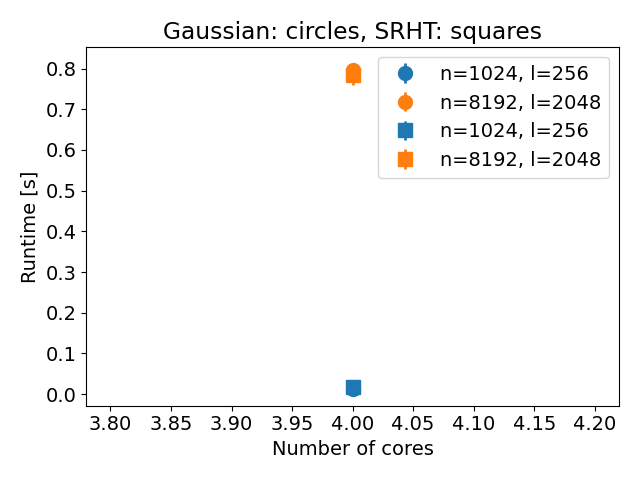
\includegraphics[width=.85\textwidth]{runtimes_cores_variation}
				\caption{Runtimes associated to the tested sketching methods as a function of the number of cores : for a ``small'' example (left) and a ``large'' one (right). Runtimes are broken down in that associated to the computation of $A\Omega,\Omega^T A\Omega$ and that associated to the computation of the $k$ rank approximation.}
				\label{fig:runtimes-cores-variation}
		\end{figure}
		- for the large : communication is not much of an issue, and big speed ups (quasi linear) are observed for the sketching computation. This means the parallelization is successful and scales well for big computations. We can see the speedup is not as good for k-rank partly because the computation was smaller to start with. The fact that the matrix is not that tall-skinny is also expected to have contributed to the low speed-up of that part.
		- 

	\section{Conclusion}
	\section*{Aknowledegments}
	\section*{References}
	%\appendix
	%	\section{Runtime Estimation}\label{appendix:runtime_estimation}
%%%
\end{document} 

